\section{Other methods}

Section that covers EA and ANN
% EA
\subsection{Evolutionary Algorithms} \label{s:lit:ea_overview}

% In the previous section described how graphs are used to analyse the gene interactions and a similar approach but the different algorithm is \acrfull{cgp}. This is part of the \acrfull{ea} family which draws inspiration from the Darwinian evolution.

\acrlong{ea} are a type of \acrshort{ml} that draws inspiration from Darwinian evolution. By incorporating random changes in the algorithm, EA can be used for optimisation or search problems. Thus, EAs are suitable for doing a wide search of the solution space\footnote{Imagine the solution space as space of the total possible solutions for a problem.} which means that they might find an unusual solution and escape the local minimum. A useful analogy here is to think as one climbing a mountain (search space), the goal (optimal solution) is to reach the highest peak but along the way, there are other peaks (local minimum) but smaller (less optimal) than the highest peak (optimal solution). The process (algorithm) of reaching the desired peak is incremental and it requires choosing the right path to the global top. Usually, an algorithm has difficulties in differentiated between the highest and lower peaks, but due to the high variation characteristic of EA, these methods perform well in such problems.


Nevertheless, these algorithms have a high computational cost and do not usually scale well, consequently being applied to relatively small problems (i.e. number of features). The corollary is that EAs are easier to understand compared to  \acrfull{dl} (explored in \cref{s:lit:dl_genomics}) and are classified as a 'white-box' approach. \Cref{s:lit:mutations} presents the MDPFinder (\citet{Zhao2012-wj}) model where \acrfull{ga}, a simpler version of EAs, are applied to process Gene Expression and mutations.

% would split the sentence here. You could then link to your next point, perhaps: "...from Darwinian evolution. By incorporating random changes in the parameters of a model, or set of models, EA can be used for optimisation..." Something like this makes it clearer why the Darwinian principles are important

As EA resembles the evolutionary process there is also some shared terminology. An individual in the EA context represents a potential solution and a population is a collection of potential solutions. \Cref{fig:ea_basic} describes the algorithmic flow of the evolutionary approach which starts with the initialisation stage, where the individuals are given (usually) random values, followed by the second stage where the fitness of the individuals is measured, that is, how suitable they are for the problem. If the problem is not solved, then it selects only the fittest individuals which are mutated, introducing variation to the new population. Similar to biology, this last step gives EA a large variety of individuals. This set of steps is run until an individual fits the solution/problem. It is worth mentioning that the mutation rate, crossover, and how the individual is selected, are preset parameters. 

\begin{figure}[!htb]
  \centering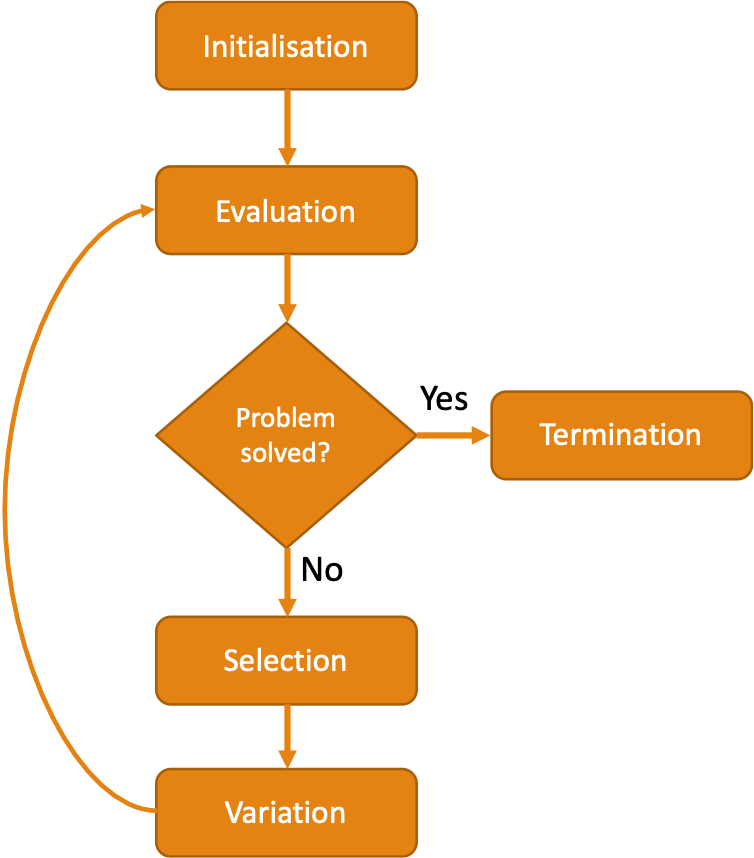
\includegraphics[width=0.4\textwidth,height=0.4\textheight,keepaspectratio]{Sections/Lit_review/Resources/EA_basic.png}
    \caption{Evolutionary Algorithms algorithm.}
    \label{fig:ea_basic}
\end{figure}
\FloatBarrier


Defining the fitness function as well as encoding the data for the EA algorithm is one of the challenges when developing EA, as it is problem-specific. The in-silico adaptation of  requires many iterations which infringes the process of scaling and has a high computational cost.

The MDPFinder model (\cref{s:lit:mutations}) used a variation of EA called \acrfull{ga} which is a simpler version of the EA family where individuals resemble the chromosome. \acrfull{cgp} is another EA algorithm which is used to process graph representation and it overcomes some of the limitations of the simpler EA methods. 

% ANN
\subsection{Artificial Neural Networks} \label{s:lit:ann_overview}

Artificial Neural Networks (ANN) are the ML strand that have been pushing the AI breakthroughs in the past 20 years. The inspiration comes from how the brain draws the information from external stimuli, stores it in its memory and retrieves it. The main components that are involved in the learning process are the neurons and the synapses between them\footnote{The neurons and synapses are the main components, but there may be others like dendrites which can also be computational units as seen later in the section.}. The simplest learning rule, introduced by Donald Hebb, states that "Neurons that fire together, wire together"\cite{Hebb_Donald1949-nn}. This means that a neuron that fires or is concurrently activated with another one (or in a given time window) forms a stronger connection. The opposite is true, the synapse weakens when two neurons do not get activated in the same time window. 

\begin{figure}[!htb]
  \centering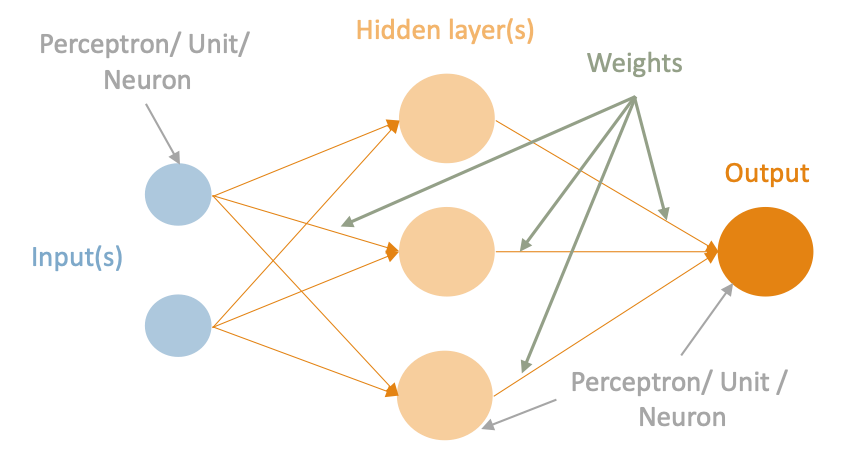
\includegraphics[width=0.7\textwidth,height=0.7\textheight,keepaspectratio]{Sections/Lit_review/Resources/Basic_ANN.png}
    \caption{A Simple ANN architecture. }
    \label{fig:ann_basic}
\end{figure}
\FloatBarrier

\Cref{fig:ann_basic} is a simple, single-layer, feed-forward Neural Network where a layer represents a collection of units that usually have the same activation function. In the case of \acrfull{dnn}, the ANN is constructed by many such layers with a large number of units. The neurons are the computational component, each having an activation function that 'tells' the unit when to activate and send a signal across the synapse. The connections between the units are assigned a weight that gives the strength of the synapses. The information is stored in the connections between the units and follows Donald Hebb's learning rule stated earlier. Therefore, the central goal of ANN is to find the specific configuration of weight values that gives the desired output. Drawing on the different types of learning mentioned earlier, in the supervised case, there is an algorithm that has been the engine of the connectionist approach called back-propagation. As the name suggests, this method propagates the input's error from the output layer back, this information is used then to compute new values for the network's weights; this is called stochastic gradient descent.

\paragraph*{Autoencoders} \label{s:lit:autoencod_overview}

Autoencoders are a particular type of Deep Neural Networks and \cref{fig:autoencoders} represents a diagram of a simple Autoencoder architecture in which there are 3 main components. The input layer to which the data is fed\footnote{The more complex version of autoencoders, including the chatGPT models, have many layers of neurons.}, and together with the output, form the encoder/decoder stages. The bottleneck part is where the data is compressed into a lower dimension. Next, a mirror to the encoder, the decoder deals with reconstructing the outputs of the bottleneck into original data. This part of autoencoders is an advantage over the PCA as the original data can be reconstructed from the lower dimension. A derivative of Neural Networks, autoencoders are more suitable to find non-linear patterns in the data whereas PCA finds only linear patterns. Given these advantageous dimension reduction techniques, it is unsurprising that there has been work done on applying Autoencoders to genomics (explored further in \cref{s:lit:autoencoders}).

\begin{figure}[!htb]
  \centering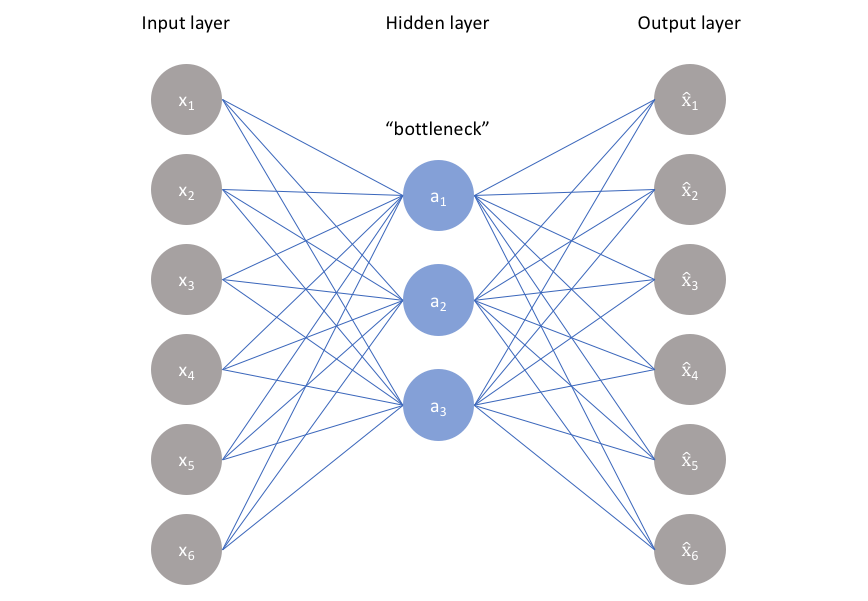
\includegraphics[width=0.8\textwidth,height=0.5\textheight,keepaspectratio]{Sections/Lit_review/Resources/simple_autoencoders.png}
    \caption{Simple architecture of autoencoders from \cite{Jordan2018-bc}}
    \label{fig:autoencoders}
\end{figure}
\FloatBarrier



Autoencoders are the most successful \acrshort{dnn} approach to problems in genomics where they have been used as a dimension reduction technique to solve the dimension curse of genetic data caused by the scarcity of samples available with a large number of features (genes). This means that they are not replacing clustering models but techniques such as \acrfull{pca} or \acrfull{nmf}, and are typically used in conjunction with clustering techniques.
